\subsection*{Problema 10}

\textbf{Enunciado:} Calcular la integral indefinida
\begin{align*}
    I = \int \dfrac{dx}{8 - 4\sin x + 7\cos x}
\end{align*}

\textbf{Solución:} Para resolver esta integral que contiene funciones trigonométricas, aplicamos la sustitución universal de Weierstrass, definida por:
\begin{align*}
    z = \tan\left(\dfrac{x}{2}\right)
\end{align*}

A partir de esta sustitución, las identidades trigonométricas fundamentales en términos de $z$ son:
\begin{align*}
    \sin x &= \dfrac{2z}{1 + z^2}, \quad 
    \cos x = \dfrac{1 - z^2}{1 + z^2}, \\
    dx &= \dfrac{2\,dz}{1 + z^2}
\end{align*}

Sustituimos estas expresiones en la integral original $I$:
\begin{align*}
    I &= \int \dfrac{\dfrac{2\,dz}{1 + z^2}}{8 - 4\left(\dfrac{2z}{1 + z^2}\right) + 7\left(\dfrac{1 - z^2}{1 + z^2}\right)}
\end{align*}

Multiplicamos el numerador y el denominador por $(1 + z^2)$ para simplificar la fracción compleja:
\begin{align*}
    I &= \int \dfrac{2\,dz}{8(1 + z^2) - 8z + 7(1 - z^2)} \\
    I &= \int \dfrac{2\,dz}{8 + 8z^2 - 8z + 7 - 7z^2}
\end{align*}

Agrupamos los términos semejantes en el denominador para obtener un trinomio cuadrático:
\begin{align*}
    I &= \int \dfrac{2\,dz}{z^2 - 8z + 15}
\end{align*}

Factorizamos el trinomio del denominador de la forma $(z - a)(z - b)$:
\begin{align*}
    z^2 - 8z + 15 &= (z - 3)(z - 5)
\end{align*}

Aplicamos el método de fracciones parciales al integrando:
\begin{align*}
    \dfrac{2}{(z - 3)(z - 5)} &= \dfrac{A}{z - 3} + \dfrac{B}{z - 5}
\end{align*}

Multiplicando por el denominador común, obtenemos:
\begin{align*}
    2 &= A(z - 5) + B(z - 3)
\end{align*}

Evaluando en los puntos críticos para hallar las constantes $A$ y $B$:
\begin{align*}
    \text{Si } z = 3 &\implies 2 = A(3 - 5) \implies A = -1 \\
    \text{Si } z = 5 &\implies 2 = B(5 - 3) \implies B = 1
\end{align*}

Sustituimos los valores de $A$ y $B$ en la integral:
\begin{align*}
    I &= \int \left( \dfrac{-1}{z - 3} + \dfrac{1}{z - 5} \right) dz
\end{align*}

Integramos cada término aplicando logaritmos naturales:
\begin{align*}
    I &= -\ln|z - 3| + \ln|z - 5| + C \\
    I &= \ln\left| \dfrac{z - 5}{z - 3} \right| + C
\end{align*}

Finalmente, regresamos a la variable original sustituyendo $z = \tan(x/2)$:
\begin{align*}
    I = \ln\left| \dfrac{\tan\left(\frac{x}{2}\right) - 5}{\tan\left(\frac{x}{2}\right) - 3} \right| + C
\end{align*}

\begin{figure}[H]
	\centering
	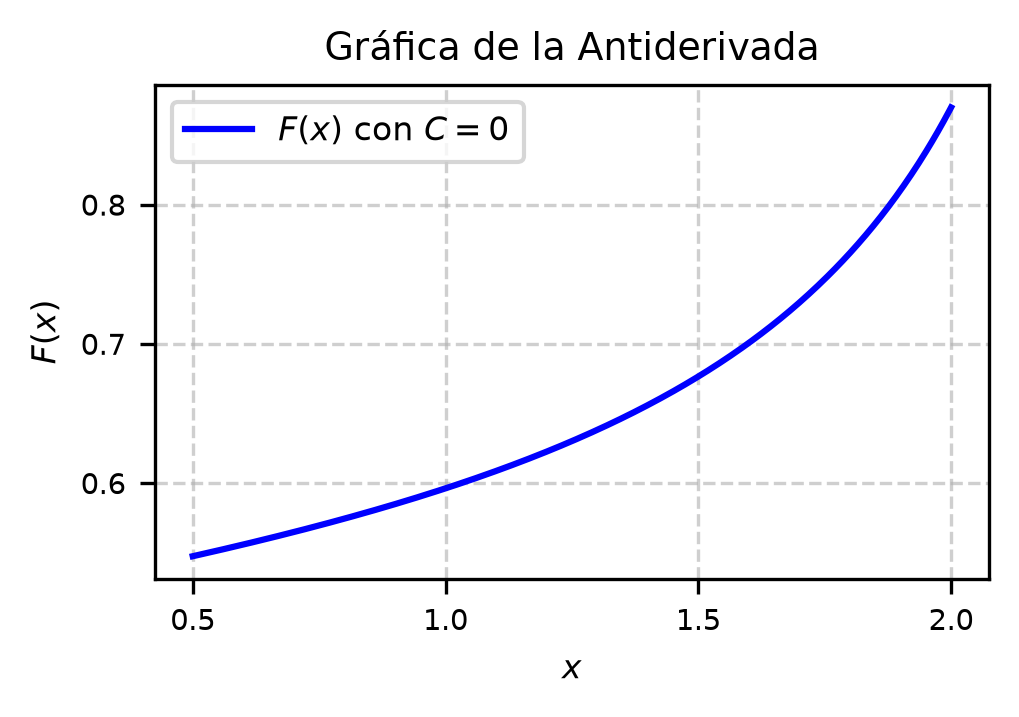
\includegraphics[width=\columnwidth]{semana_04/graficas/SEM04_P10_grafica.png}
	\caption{Representación gráfica de $f(x)$ y su antiderivada $F(x)$ evaluada para la constante de integración $C = 0$ (Problema 10).}
	\label{fig:problema10}
\end{figure}
